\documentclass[a4paper,12pt]{article}


\usepackage{setspace}

\usepackage[T1]{fontenc} % Codificacao da fonte
\usepackage{times} % Definindo a fonte como Times New Roman

\usepackage{fancyhdr}
\pagestyle{fancy}
\lhead{Centro Universitário da FEI}

\rfoot{\thepage} %número da página
\cfoot{\textit{[ELC220] Controle Digital}}

\usepackage[left=2cm,right=2cm,top=2cm,bottom=2cm]{geometry}

\usepackage[utf8]{inputenc}


\usepackage{graphicx}
\usepackage{float}
\usepackage{amsmath}
\usepackage{gensymb}

\begin{document}
	\begin{center}
		\begin{Huge}
			Atividade Parcial
		\end{Huge}
	\end{center}

	\begin{center}
		\centering{\textbf{Gustavo Rosell Collado (11.121.526-5)}}\\
		\centering{\textbf{Massiel Blandy Ramón (11.122.397-0)}}\\
		\centering{\textbf{Thiago Travagini Moura (11.121.329-4)}}
		
		
		
	\end{center}
	
	\paragraph{}
	
	\section{Problema 1}
	Uma câmara térmica usada para testes de stress térmico em grandes equipamentos é mostrada na figura 1 com seu respectivo diagrama de blocos simplificado. Considere a unidade de tempo em minuto. A câmara é aquecida por uma linha de vapor que é controlada por uma válvula eletricamente ativa. A abertura da porta afeta a temperatura da câmara e pode ser considerada como um distúrbio. No diagrama de blocos d(t) é um distúrbio causado pela abertura da porta, e(t) é o sinal de entrada do sistema e c(t) a temperatura de saída na câmara térmica.
	

	\begin{figure}[H]
		\centering
		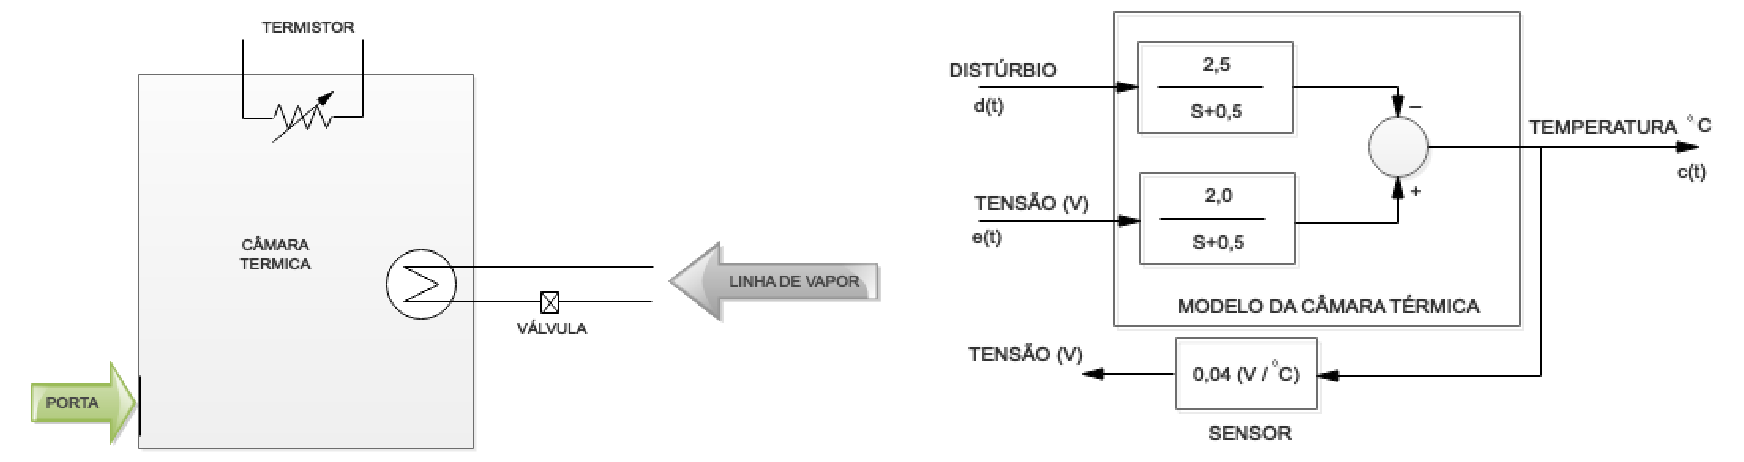
\includegraphics[width=0.9\linewidth]{images/planta_problema1}
		\label{fig:plantaproblema1}
	\end{figure}

	\subsection{Constante de tempo da câmara}
		Para analisarmos qual a constante de tempo do sistema, podemos compara-la a forma genérica da função de sua respectiva ordem, onde nesse caso é um sistema de primeira ordem. Como mostra a equação abaixo é possível obter qual a constante de tempo.
	
		\begin{equation}
			\left.
			\begin{array}{c}
				\displaystyle G(s) = \frac{K}{s+a} \\[20pt]
				\displaystyle \tau = \frac{1}{a}
			\end{array}
			\right\}
			\quad \tau = \frac{1}{0,5} = 2
		\end{equation}
	
		Portanto para câmara proposta a constante de tempo $\tau$ é 2 minutos, portanto o tempo de subida desse ($T_s$) sistema será $4 \cdot \tau = 8$ minutos.
	
	\subsection{Resposta da câmara com condição inicial zero e sem distúrbio}
		Considerando a porta da câmara fechada (sem distúrbio) e com condição inicial 0\degree C, sendo a entrada de sinal um degrau de amplitude cinco tem-se então:
		

		\begin{gather}
			C(s) = \frac{2,0}{s+0,5} \cdot \frac{5,0}{s} = \frac{10,0}{s^2 + 0,5s} = \frac{20}{s} - \frac{20}{s+0,5} \\[20pt]
			c(t) = \mathcal{L}^{-1} \{ C(s) \} = 20 + 20e^{-0,5t}
		\end{gather}
	
		Utilizando o \textit{MATLAB} foi obtido o seguinte gráfico:
		
		\begin{figure}[H]
			\centering
			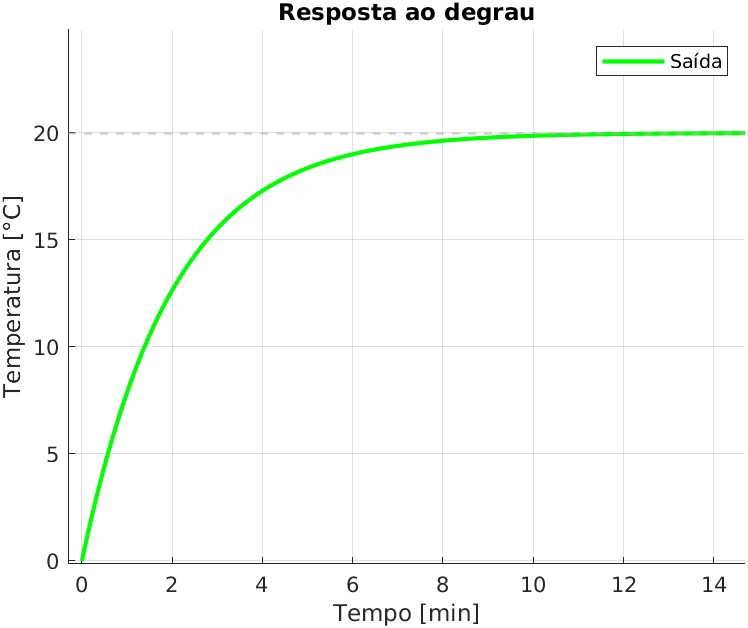
\includegraphics[width=0.5\linewidth]{images/respb.png}
			\label{fig:resposta_b}
		\end{figure}
	
		É possível observar que para essa entrada degrau de amplitude 5 o sistema, para $t$ tendendo ao infinito, estabiliza em 20\degree C.
		
	\subsection{Resposta da câmara com condição inicial 25\degree C e sem distúrbio}
		Sendo feita o mesmo procedimento que o item anterior, porém adicionando uma condição inicial, pode-se dizer que a única mudança será:
		
		\begin{equation}
			c(t) = c_{Anterior}(t) + x_0 \rightarrow c(t) = 45 + 20e^{-0,5t}
		\end{equation}
	
		E com essa equação tem-se o seguinte gráfico.
		
		\begin{figure}[H]
			\centering
			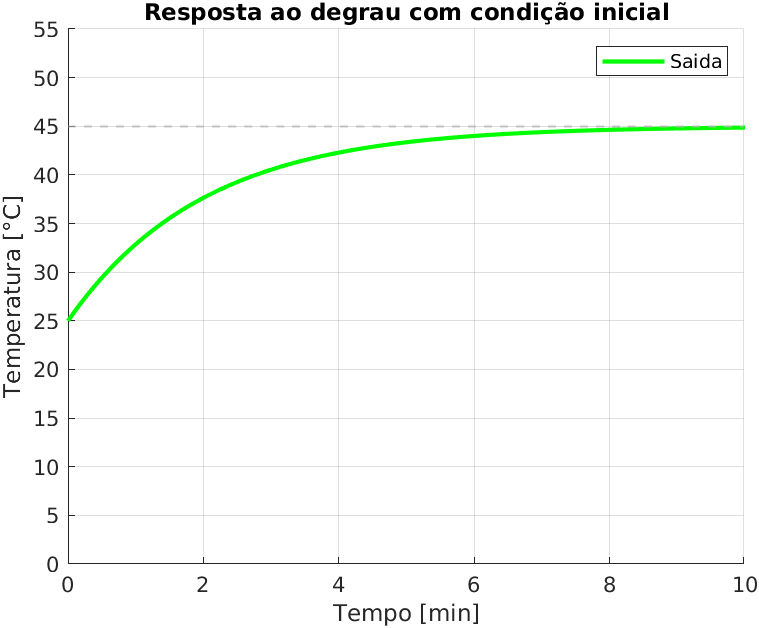
\includegraphics[width=0.5\linewidth]{images/respc.png}
			\label{fig:resposta_c}
		\end{figure}
	
	\subsection{Resposta da câmara com condição inicial 25\degree C e com distúrbio continuo}
		Nesse novo cenário é estudado como se comporta a planta para uma entrada degrau de amplitude 5, com condição inicial de 25\degree C e para um distúrbio com uma entrada de degrau unitário após 2 minutos do inicio, tem-se que:
		
		\begin{gather}
			C(s) = G(s) \cdot E(s) - G_d(s) \cdot D(s)  + X_0(s)\\[20pt]
			C(s) = \frac{2,0}{s+0,5} \cdot \frac{5,0}{s} - \frac{2,5}{s+0,5} \cdot \frac{e^{-2s}}{s} + X_0(s) \\[20pt]
			c(t) = \mathcal{L}^{-1} \{ C(s) \} = 20 - 20e^{-0,5t} - (5 - 5e^{-0,5(t-2)})u(t-2) + 25 \\[20pt]
			c(t) = 45 - 20e^{-0,5t} - (5 - 5e^{-0,5(t-2)})u(t-2)
		\end{gather}
	
		Para essas condições a resposta do sistema foi:
		
		\begin{figure}[H]
			\centering
			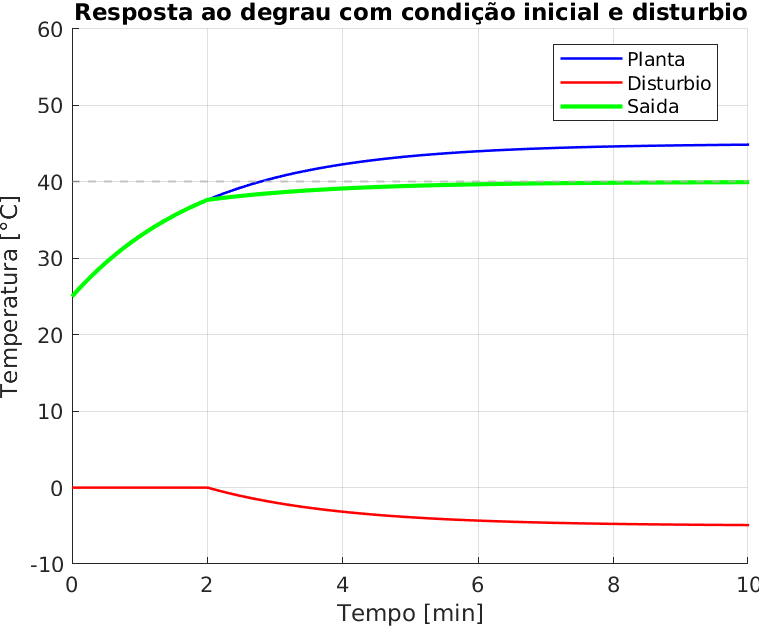
\includegraphics[width=0.5\linewidth]{images/respd.png}
			\label{fig:resposta_d}
		\end{figure}
	
		Do gráfico é possível observar o momento em que o distúrbio começa, em 2 minutos, e o valor final desse distúrbio que é de -5\degree C.
		
	\subsection{Resposta da câmara com condição inicial 25\degree C e com distúrbio finito}
		Nesse ultimo cenário é o mesmo utilizado acima porém com a interrupção do distúrbio apos 12 minutos do seu inicio portanto para obtermos $c(t)$ basta adicionarmos essa interrupção na resposta anterior e a função sera:
		
		\begin{equation}
			c(t) = 45 - 20e^{-0,5t} - (5 - 5e^{-0,5(t-2)})u(t-2) + (5 - 5e^{-0,5(t-14)})u(t-14)
		\end{equation}
	
		E sua resposta foi:
		
		\begin{figure}[H]
			\centering
			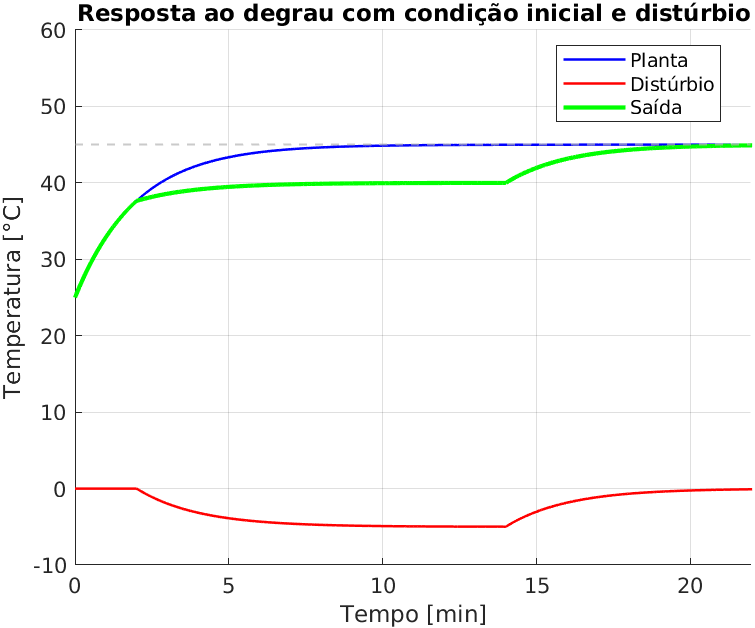
\includegraphics[width=0.5\linewidth]{images/respe.png}
			\label{fig:resposta_e}
		\end{figure}
	
	\section{Problema 2}
		% TODO: Colocar a citação da figura e todos os captions das figuras
		A figura 2 mostra o sistema de controle de temperatura da câmara térmica do problema 1.
		
		\begin{figure}[H]
			\centering
			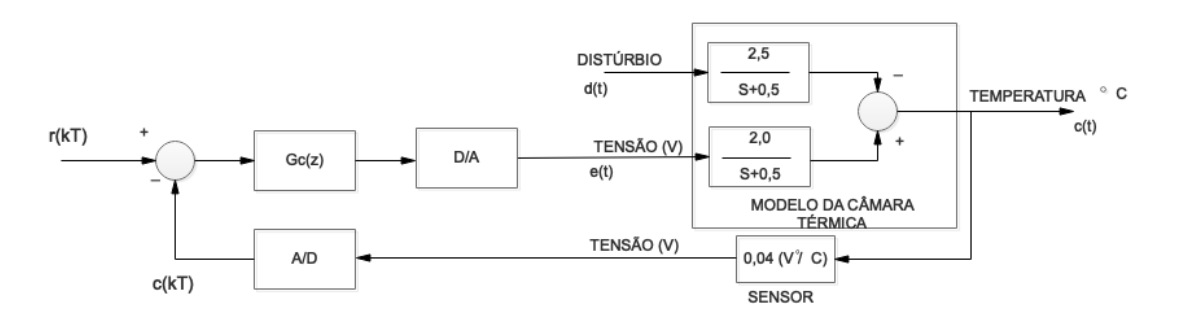
\includegraphics[width=0.9\linewidth]{images/planta_problema2}
			\label{fig:plantaproblema2}
		\end{figure}
	
		\subsection{Função de transferência no domínio z}
			Para obter a função de transferência no domínio z, é necessário inicialmente converter a planta e os conversores para o domínio z. Com $T=0,6$ min temos:
		
			\begin{equation}
				\left.
				\begin{array}{c}
					\displaystyle H(z) = (1 - z^{-1}) \cdot Z\left[\frac{G(s)}{s}\right] \\[20pt]
					
					\displaystyle Z\left[\frac{G(s)}{s}\right] = Z\left[\frac{2,0}{s(s+0,5)}\right] = 4 \cdot Z\left[\frac{0,5}{s(s+0,5)}\right] = 4 \cdot \frac{(1 - e^{-0,5T})z}{(z-1)(z-e^{-0,5T})} \\[20pt]
					\displaystyle H(z) = \frac{z-1}{z} \cdot 4 \cdot \frac{(1 - e^{-0,5T})z}{(z-1)(z-e^{-0,5T})} = \frac{4(1 - e^{-0,5T})}{(z-e^{-0,5T})} = \frac{1,037}{(z-0,741)}
				\end{array}
				\right.
				\quad 
				\label{eq:hz06}
			\end{equation}
			
			% TODO: rever o nome diagrama de blocos e incluir aqui
			Portanto tem-se um sistema representado pelo seguinte diagrama de blocos.
			
			
			E a função de transferência de malha fechada será igual:
			
			\begin{equation}
				\left.
				\begin{array}{c}
					\displaystyle \frac{C(z)}{R(z)} = \frac{G_C(z) \cdot \displaystyle \frac{1,037}{(z-0,741)}}{1 + \cdot G_C(z) \cdot \displaystyle \frac{1,037}{(z-0,741)} \cdot 0,04} = \frac{G_C(z) \cdot 1,037}{z - 0,741 + G_C(z) \cdot 0,041}
				\end{array}
				\right.
				\quad 
				\label{eq:ftma}
			\end{equation}
		
		\subsection{Distúrbio no domínio z}
			Admitindo a entrada $r(kT)=0$ o sistema em malha aberta é possível extrair a temperatura $c(t)$ quando há um distúrbio com uma entrada de degrau unitário. 
			
			\begin{equation}
				\left.
				\begin{array}{c}
					\displaystyle C_d(z) = G_d(z) \cdot D(z) = Z\left[\frac{2,5}{s+0,5} \cdot \frac{1}{s} \right] = 5 \cdot Z\left[\frac{1}{s(s+0,5)} \right] \\[20pt]
					\displaystyle C_d(z) = 5 \cdot \frac{(1 - e^{-0,5T})z}{(z-1)(z-e^{-0,5T})} = \frac{01,296z}{(z-1)(z-0,741)}
				\end{array}
				\right.
				\quad 
			\end{equation}
			
		\subsection{Expressão completa do sistema}
			Para obter a expressão completa do sistema é necessário considerado uma entrada $r(kT)$ genérica e um distúrbio que ocorre num instante n. Dessa forma tem-se:
			
			\begin{equation}
				\left.
				\begin{array}{c}
					\displaystyle C(z) = \frac{G_C(z) \cdot 1,037}{z - 0,741 + G_C(z) \cdot 0,041} \cdot Z\left[r(kT)\right] - \frac{1,296z}{(z-1)(z-0,741)} \cdot z^{-n}
				\end{array}
				\right.
				\quad 
			\end{equation}
	
		\subsection{Cenário 1}
		
			Admitindo um período de amostragem $T = 0,6$ min e $Gc(z) = 1,0$, a equação de diferenças para c(kT) quando é aplicado um degrau r(kT) = 0,4 h(kT) resulta em:
			
			\begin{equation}
				\left.
				\begin{array}{c}
					\displaystyle C(z) = \frac{1,0 \cdot 1,037}{z - 0,741 + 1,0 \cdot 0,041} \cdot Z\left[r(kT)\right] = \frac{1,037}{z - 0,7} \cdot R(z)
				\end{array}
				\right.
				\quad 
			\end{equation}
			
			Normalizando tem-se:
			
			\begin{equation}
				\left.
				\begin{array}{c}
					\displaystyle C(z) = \frac{1,037}{z - 0,7} \cdot R(z) = \frac{1,037 \cdot z^{-1} \cdot R(z)}{1 - 0,7 \cdot z^{-1}}  \rightarrow \\[20pt]
					\rightarrow \displaystyle c(kT) = 0,7\cdot c[(k-1)T] + 1,037 \cdot r[(k-1)T]
				\end{array}
				\right.
				\quad 
			\end{equation}
			
			Para se obter qual o valor, em temperatura, para uma entrada degrau com amplitude de 0,4, basta admitir que para esse valor final o erro deve ser nulo portanto:
			
			\begin{equation}
				\left.
				\begin{array}{c}
					\displaystyle e(t)= r(t) - c(t) = 0 \rightarrow c(t) \cdot 0,04 = r(t) \rightarrow c(t) = \frac{0,4}{0,04} = 10 \celsius
				\end{array}
				\right.
				\quad 
			\end{equation}
			
			Utilizando também o teorema do valor final tem-se:
			
			\begin{equation}
				\left.
				\begin{array}{c}
					\displaystyle \lim_{k \to \infty}f(k) = \lim_{z \to 1}\left[(1-z^{-1})F(z) \right] \rightarrow \lim_{k \to \infty}f(k) = \lim_{z \to 1}\left[ \frac{z-1}{z} \cdot \frac{1,037}{z - 0,7} \cdot 0.4 \cdot \frac{z}{z-1}  \right] \rightarrow \\[20pt]
					
					\displaystyle \rightarrow \lim_{k \to \infty}f(k) =  \lim_{z \to 1}\left[  \frac{0,415}{z - 0,7}  \right] = 1,383
				\end{array}
				\right.
				\quad 
			\end{equation}
			
			Nessa situação temos um sistema estável porém com erro de aproximadamente 86,2\%
			
			
		\subsection{Erro cenário 1}
			
			\begin{equation}
				\left.
				\begin{array}{c}
					\displaystyle e(kT) = r(kT) - 0,04 \cdot c(kT) \rightarrow \\[20pt]
					\displaystyle \rightarrow e(kT) = r(kT) - 0,04 \cdot (0,7\cdot c[(k-1)T] + 1,037 \cdot r[(k-1)T]) \rightarrow \\[20pt]
					\displaystyle \rightarrow e(kT) = r(kT) - 0,028 \cdot c[(k-1)T] - 0,041\cdot r[(k-1)T]
				\end{array}
				\right.
				\quad 
			\end{equation}
			
		\subsection{Sistema com ganho infinito}
			Observando a equação \ref{eq:ftma} fica visível que os polos do sistema tem relação direta com o controlador, para um valor de K muito alto o polo do sistema estará fora do circulo de raio unitário do plano z, portanto esse sistema sera instável.
			
		\subsection{Alterando o período de amostragem}
			Supondo um periodo de amostragem de $T = 6$ mim eh necessario refazer alguns calculos sendo inicialmente o calculo de $H(z)$ realizado na equacao \ref{eq:hz06}.
			
			\begin{equation}
			\left.
			\begin{array}{c}
				\displaystyle H(z) = (1 - z^{-1}) \cdot Z\left[\frac{G(s)}{s}\right] \\[20pt]
				
				\displaystyle H(z)  = \frac{4(1 - e^{-0,5T})}{(z-e^{-0,5T})} = \frac{3,801}{(z-0,050)}
			\end{array}
			\right.
			\quad 
		\end{equation}
		
		Na sequencia se obtém a função de transferência de malha fechada.
		
		\begin{equation}
			\left.
			\begin{array}{c}
				\displaystyle \frac{C(z)}{R(z)} = \frac{G_C(z) \cdot \displaystyle \frac{3,801}{(z-0,050)}}{1 + \cdot G_C(z) \cdot \displaystyle \frac{3,801}{(z-0,050)} \cdot 0,04} = \frac{G_C(z) \cdot 3,801}{z - 0,050 + G_C(z) \cdot 0,152} \rightarrow \\[30pt]
				
				\displaystyle \rightarrow \frac{C(z)}{R(z)} = \frac{3,801}{z + 0,102}
			\end{array}
			\right.
			\quad 
			\label{eq:ftma}
		\end{equation}
		
		Utilizando o teorema do valor final
		
		\begin{equation}
			\left.
			\begin{array}{c}
				\displaystyle \lim_{k \to \infty}f(k) = \lim_{z \to 1}\left[(1-z^{-1})F(z) \right] \rightarrow \lim_{k \to \infty}f(k) = \lim_{z \to 1}\left[ \frac{z-1}{z} \cdot \frac{3,801}{z + 0,102} \cdot 0.4 \cdot \frac{z}{z-1}  \right] \rightarrow \\[20pt]
				
				\displaystyle \rightarrow \lim_{k \to \infty}f(k) =  \lim_{z \to 1}\left[  \frac{1,520}{z + 0,102}  \right] = 1,380
			\end{array}
			\right.
			\quad 
		\end{equation}	
		
		Utilizando o software MATLAB foi possível obter a resposta do sistema
		
		\begin{figure}[H]
			\centering
			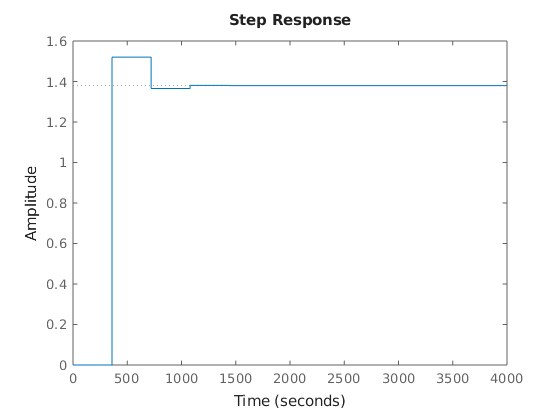
\includegraphics[width=0.5\linewidth]{images/resp2g.png}
			\label{fig:resposta_e}
		\end{figure}
		
				

			
			
			
			
			
			
		
		
		
		
		
		
		
		
		
		
		
	
	
\end{document}